\chapter{検証実験}
\thispagestyle{empty}
\label{chap3}
\minitoc

\newpage
%%%%%%%%%%%%%%%%%%%%%%%%%%%%%%%%%%%%%%%%%%%%%%%%%%%%%%%%%%%%%%%%%%%%%%%%%%%%%%%
%==============================================================================
%はじめに
%==============================================================================
\section{はじめに}
本章では,第 2 章で述べた提案手法の有効性を検証するために行った実験について述
べる.
\par
3.2 では,模型による3次元物体検出の実験と結果について述べる.
\par
3.3 では,実機による実験に使用した装置の構成,計測対象,実験方法について述べる.
\par
3.4 では,提案手法による処理結果,位置姿勢推定の結果について述べる.
\newpage

\section{模型による3次元物体検出の実験}
\subsection{実験環境}
本節では,模型による3次元物体検出の実験に使用したデータセットの作成環境と実験方法について述べる.図\ref{fig:tr}に示すように,データセットの作成には,回転台,ダンプトラックの模型とRGB-Dを使用した.
回転台は,ComXimのターンテーブル(\ref{fig:table}),ダンプトラックの模型(\ref{fig:truck})は,プラッツの1/50日野プロフィア(\ref{tab:truck}),RGB-Dセンサは,IntelのRealSense D435i(\ref{tab:intel}) を使用した.表\ref{tab:table},
表\ref{tab:truck},表\ref{tab:intel}
にそれぞれ,回転台,模型とRGB-Dセンサの仕様を示す.RGB-Dセンサは,内蔵したIMUにより取得した姿勢を基に地面に並行となるようにセンサ座標を座標変換する.
\begin{figure}[b]
    \begin{center}
    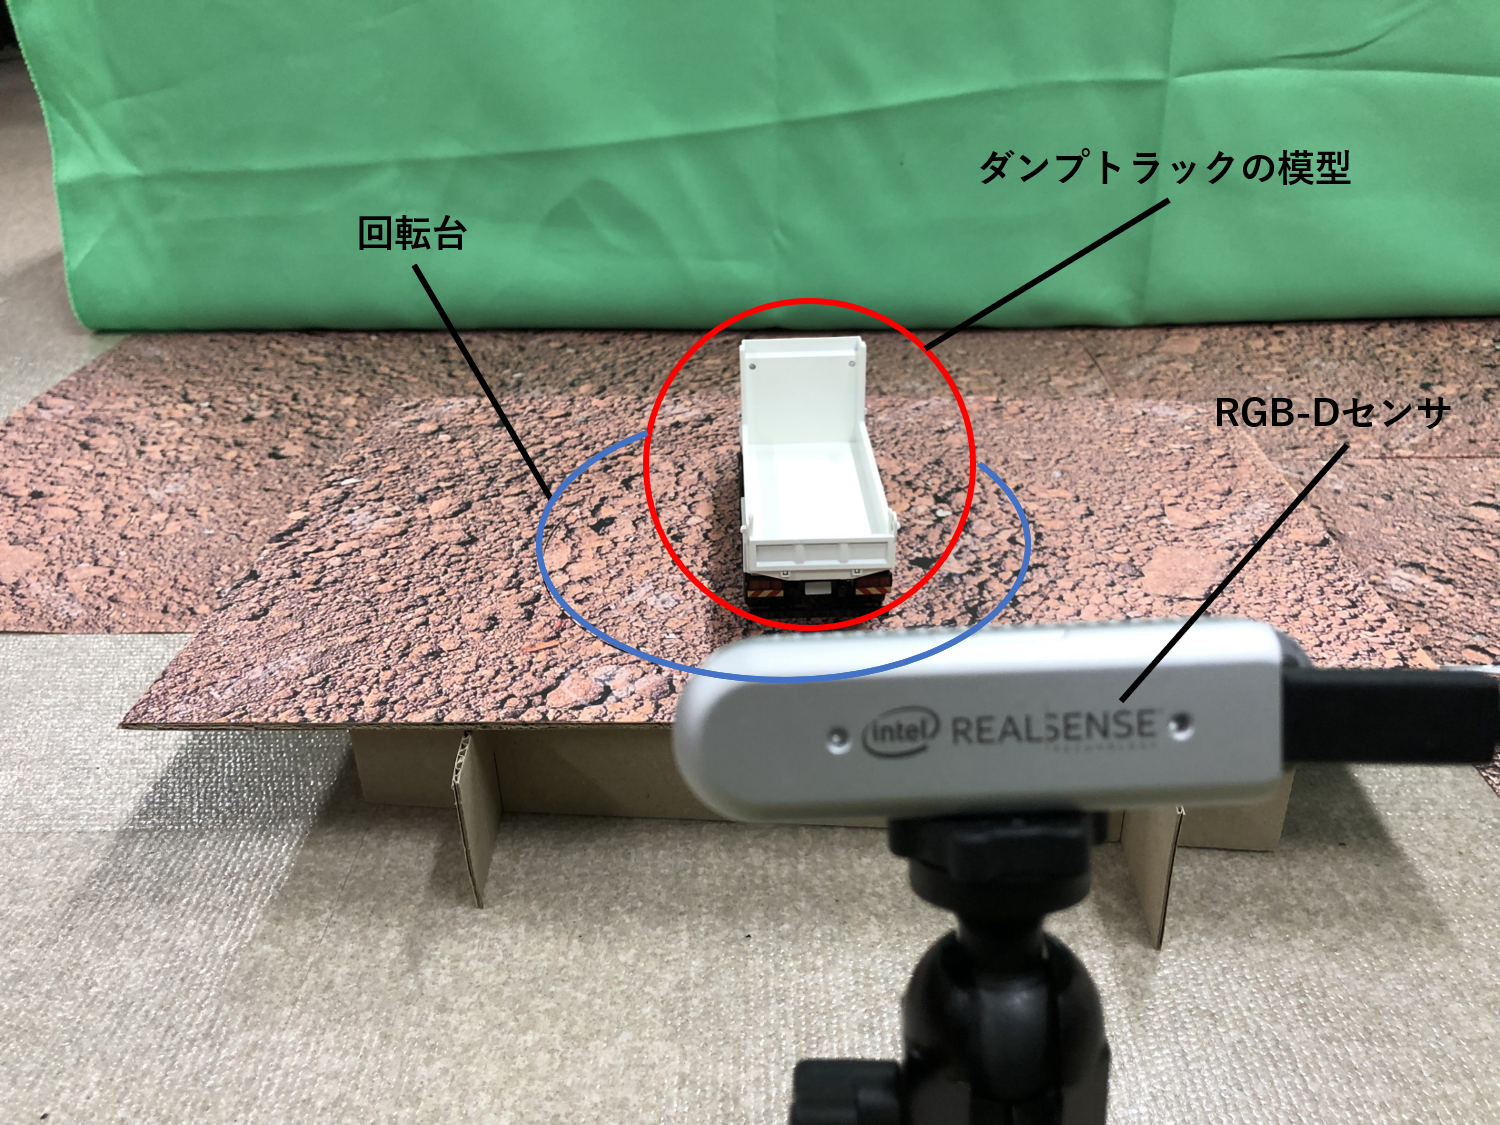
\includegraphics[width=0.5\columnwidth]{./chap3/fig/train.eps}
    \caption{撮影環境}
    \label{fig:tr}
    \end{center}
    %\vspace{-5mm}
\end{figure}

\begin{figure}[b]
    \begin{minipage}{0.5\hsize}
     \begin{center}
      \includegraphics[width=45mm]{./chap3/fig/table.eps}
     \end{center}
     \caption{ComXim ターンテーブル}
     \label{fig:table}
    \end{minipage}
    \begin{minipage}{0.5\hsize}

    \begin{center}
     \includegraphics[width=45mm]{./chap3/fig/truck.eps}
    \end{center}
     \caption{プラッツ 1/50日野プロフィア}
     \label{fig:truck}
    \end{minipage}
    
\end{figure}
\clearpage

\begin{figure}[b]
    \begin{center}
    \includegraphics[width=0.4\columnwidth]{./chap3/fig/intel.eps}
    \caption{IntelのRealSense D435i}
    \label{fig:intel}
    \end{center}
    %\vspace{-5mm}
\end{figure}

\begin{table}[b]
    \begin{center}
    \caption{ComXim ターンテーブル}
    \begin{tabular}{|c|c|}
    \hline
    最大耐荷重     & 20 kg   \\ \hline
    角度分解能     & 0.1 deg \\ \hline
    外形寸法(R x H) & 20 x 5 cm \\ \hline
    質量        & 0.8 kg  \\ \hline
       \end{tabular}
    \label{tab:table}
    \end{center}
\end{table}

\begin{table}[b]
    \begin{center}
    \caption{プラッツ 1/50日野プロフィア}
    \begin{tabular}{|c|c|}
    \hline
    外形寸法(L x W x H) & 160 x 60 x 71 mm \\ \hline
    質量          & 281 g        \\ \hline
    \end{tabular}
    \label{tab:truck}
    \end{center}
\end{table}

\begin{table}[b]
    \begin{center}
    \caption{Intel RealSense D435i}        
\begin{tabular}{|c|c|}
\hline
解像度(W x H)      & 1280 x 720               \\ \hline
動作範囲      & 0.1 $\sim$ 10 m            \\ \hline
Depth 視野角 & 87° x 58° x 95° \\ \hline
RGB 視野角   & 69° x 42° x 77°      \\ \hline
IMU       & BMI055                   \\ \hline
    \end{tabular}
    \label{tab:intel}
    \end{center}
\end{table}

\clearpage

\subsection{検証結果}
\section{実機による実験}
\subsection{実験環境}
\subsection{実験方法}
\section{実機による実験の結果}
\subsection{ダンプトラックの点群抽出の結果}
\subsection{位置姿勢推定の結果}
\section{おわりに}
